\section{Fiji VM}
I linguaggi più utilizzati, in genere, per sistemi real-time sono Ada e C (per i più coraggiosi C++). Tuttavia la complessità e la dimensione crescente del codice, unita alla disponibilità di tanti programmatori ben addestrati hanno portato fatto crescere l'interesse verso l'utilizzo di Java. Inoltre, dato che le applicazioni Android sono generalmente scritte in Java, per poter utilizzare quei dispositivi in contesti con vincoli temporali è necessario avvicinare il mondo Java e quello real-time. Per farlo è necessario sviluppare un runtime, e una GC, che siano prevedibili e adatti all'utilizzo in sistemi con vincoli temporali stretti. La Fiji VM (fVM) ha esattamente questo scopo. Figura~\ref{fig:fijiarch} mostra la sua architettura.
\begin{figure}
	\centering
	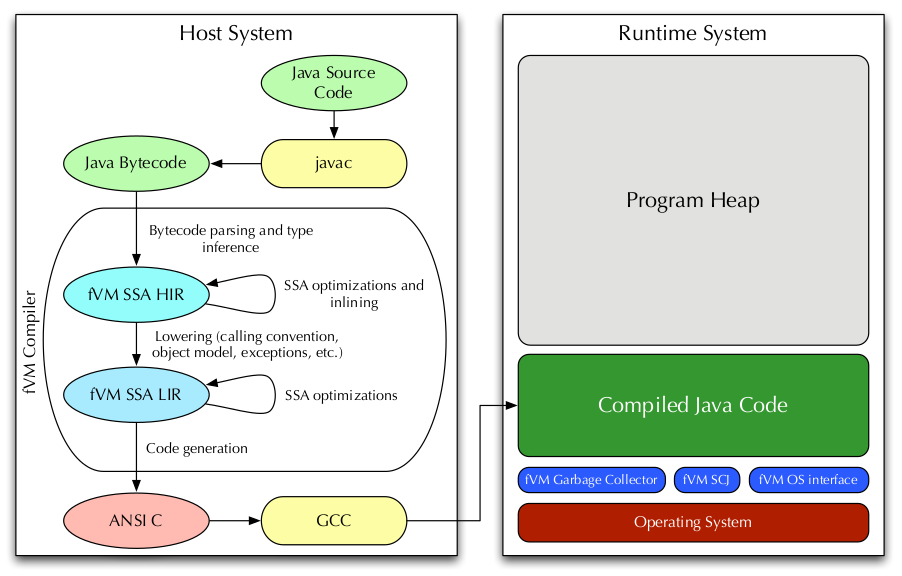
\includegraphics[width=0.9\linewidth]{fijiarch}
	\caption[Architettura di Fiji VM]{Architettura di Fiji VM}
	\label{fig:fijiarch}
\end{figure}

\subsection{Compilazione}
fVM utilizza un compilatore AOT per convertire codice Java in ANSI C. A partire dal codice Java vengono inizialmente effettuate diverse ottimizzazioni basate sulla rappresentazione static-single-assignment (SSA); tra queste troviamo:
\begin{itemize}
	\item inlining;
	\item devirtualizzazione (chiamate virtuali tradotte in chiamate dirette;
	\item virtualizzazione (chiamate di interfaccia in chiamate virtuali);
	\item eliminazione dei lock (se si sa che un lock è attivo non serve fare avere codice che lo attiva nuovamente);
	\item eliminazione dei controlli sulle dimensioni degli array e sui null pointers;
	\item copy propagation.
\end{itemize}
Di seguito vengono descritte le modalità di compilazione.

\paragraph{Null pointers} \mbox{} \\
Java controlla che ogni puntatore sia non null prima di utilizzarlo. Attraverso tecniche di analisi del flusso di controllo è possibile eliminare questi controlli ed evitare percorsi di esecuzione diversi con tempi diversi.

\paragraph{Dimensione degli array} \mbox{} \\
Così come per i controlli sui puntatori nulli, anche i controlli sugli indici degli array possono essere rimossi per evitare di incorrere in incrementi del tempo di esecuzione.

\paragraph{Controlli per la garbage collection} \mbox{} \\
Dato che il GC opera concorrentemente all'applicazione (= non la mette in pausa), è necessario fare alcuni controlli a run-time:
\begin{itemize}
	\item \textbf{sync-points}: indicano che lo stack del thread corrente deve essere analizzato dal GC;
	\item \textbf{stone barriers}: assicurano che le modifiche fatte allo heap siano viste dal GC.
\end{itemize}
I primi sono inseriti utilizzando una politica che assicura una distanza limitata tra due diversi punti. Questo significa che ogni ciclo ne avrà almeno uno. L'impatto sui cicli ''snelli'' è significativo, perché viene introdotto un nuovo branch. Tuttavia i test effettuati mostrano che, in generale, l'overhead è trascurabile. fVM mantiene un puntatore ad una struttura dati corrispondente allo del thread corrente. Questa struttura contiene un campo, \texttt{shouldSync}, che è \texttt{true} quando il thread deve sincronizzarsi (\texttt{yield()}). I thread con alta priorità, tale da poter prerilasciare il GC, non sono affetti da questo controllo, ma tutti gli altri subiranno un overhead inevitabile. 

Le seconde introducono un altro overhead nella pulizia, e vengono tradotte nel modo seguente (per ogni modifica ad un puntatore):
\begin{lstlisting}[caption={Stone-barrier},label={lst:stone}]
if (source != null && source.gcState != marked)
	mark(source);
target.field = source;
\end{lstlisting}
Il primo controllo è spesso rimosso (in virtù di quanto detto prima), ma comunque i due percorsi avranno tempi di esecuzione diversi (rallentamento se la condizione è vera).

\paragraph{Variabili locali} \mbox{} \\
La maggior parte delle assegnazioni di variabili locali sono eliminate attraverso copy propagation o tradotte in assegnazioni C. Questo non vale se le variabili contengono puntatori. Infatti i compilatori C non forniscono metodi adeguati per analizzare lo stack, operazione necessaria per la GC. Il problema viene risolto utilizzando una struttura allocata sullo stack che contiene copie a tutti i riferimenti locali allo heap. In questo modo è possibile sempre avere la situazione dei riferimenti locali sotto controllo, senza impattare significativamente le performance.

\paragraph{Invocazione di metodi} \mbox{} \\
L'invocazione dei metodi è tradotta in una chiamata di funzione C. Ci sono vari overhead indiretti legati alla gestione della struttura dati per la GC e al controllo delle eccezioni. Per ovviare a questi problemi vengono effettuate ottimizzazioni di inlining e devirtualizzazione molto aggressive. I metodi piccoli o quelli chiamati molto spesso (a meno che non siano \textit{troppo} grandi) vengono aggiunti inline. I metodi ricorsivi sono penalizzati, perché l'inlining ricorsivo viene evitato, ma gli altri raggiungono velocità pari agli equivalenti C.

\paragraph{Inizializzazione statica} \mbox{} \\
Java aggiunge controlli sull'inizializzazione delle classi prima di ogni chiamata di un metodo statico, di ogni accesso ad un campo statico e di ogni istanziazione. I controlli ridondanti possono essere rimossi analizzando il flusso di controllo. Le librerie sono state inoltre progettate per fare un uso minimo dell'inizializzazione statica o per permettere alla VM di inizializzare il più possibile prima dell'esecuzione. Tali controlli possono quindi essere rimossi dal compilatore.

\paragraph{Allocazione} \mbox{} \\
Per allocare memoria viene fatto un primo tentativo con del codice C per salvare l'oggetto nella prima posizione raggiungibile. Se l'allocazione fallisce, si cerca la prima posizione disponibile. Il GC agisce in modo concorrente, ma ci possono essere dei casi nei quali l'applicazione è costretta a mettersi in pausa in attesa del completamento della pulizia (se la memoria è piena). L'intera procedura è al più tanto lenta quanto una chiamata C \texttt{malloc}. 

\paragraph{Sincronizzazione} \mbox{} \\
Viene utilizzato codice C per acquisire velocemente il lock e codice specifico per permettere la gestione dei lock rispettando RTSJ. I lock del SO sono utilizzati internamente, e l'implementazione è molto più efficiente rispetto a quella ottenuta utilizzando solamente C.

\subsection{Garbage Collection}
Esistono principalmente tre famiglie di algoritmi di GC:
\begin{itemize}
	\item \textbf{Sweep-to-free-list}: basano l'intero processo di allocazione/rimozione su una lista di posizioni libere. Strategie di questo tipo sono dette \textit{non-moving}, nel senso che gli oggetti non vengono mai spostati una volta allocati. Per questo sono molto efficienti in termini di tempo e spazio, ma non forniscono località agli oggetti allocati. Un esempio sono gli algoritmi \textbf{mark-sweep};
	\item \textbf{Evacuation}: spostano tutti gli oggetti attivi in un nuovo spazio, reclamando tutto il vecchio spazio in un colpo solo. Alcuni esempi sono: \textbf{semi-space}, \textbf{older-first}, \textbf{garbage-first};
	\item \textbf{Compaction}: spostano tutti gli oggetti vivi ad un'estremità dello \textit{stesso} spazio, reclamando lo spazio restante in un colpo solo. Un esempio sono gli algoritmi \textbf{mark-compact}.
\end{itemize}
Gli ultimi due forniscono allocazione contigua e quindi offrono all'applicazione la località degli oggetti memorizzati. Tuttavia occupano generalmente il doppio dello spazio, e compattare è inefficiente perché richiede più passate dello heap.

Una categoria alternativa è data dagli algoritmi \textbf{mark-region}. Questi utilizzano una strategie non-moving e \textbf{sweep-to-region}, che libera zone contigue di memoria e quindi fornisce un miglior grado di allocazione contigua: per ridurre la frammentazione viene fatta una deframmentazione opportunistica. In questo modo è possibile ottenere un algoritmo efficiente in termini di spazio e tempo, con allocazione continua. Il problema è dimensionare correttamente le regioni: regioni grandi massimizzano le performance dell'applicazione e minimizzano il costo di pulizia, ma sono onerose in termini di spazio (un solo oggetto puù bloccare l'intera regione); regioni piccole, invece, aumentano l'efficienza spaziale, ma aumentano il tempo di pulizia della memoria e riducono le prestazioni dell'applicazione. Inoltre, con regioni piccole, la marcatura degli oggetti è più onerosa. Un algoritmo di questo tipo è \textit{Immix}. Fiji utilizza una versione leggermente modificata di quest'ultimo.

\subsubsection{Immix}
Implementare in modo ingenuo un algoritmo mark-region è molto facile: la memoria è divisa in zone di dimensione fissata, che possono essere libere o allocate. Durante l'allocazione vengono riempite le regioni disponibili fino a quando la memoria non è esaurita. A quel punto parte la collection. Vengono quindi marcate tutte le regioni con oggetti attivi come non disponibili, e tutte le altre come libere. Gli oggetti, inoltre, non possono estendersi su più regioni. 

Un approccio di questo tipo evidenzia due problemi. Il primo riguarda il dimensionamento delle regioni. Il secondo riguarda la deframmentazione: una regione è non disponibile fintanto che contiene un oggetto vivo, quindi è necessario deframmentare per recuperare più memoria.

Immix risolve il problema operando a due livelli: \textbf{blocchi} e \textbf{linee}. Quando, durante l'allocazione, viene riciclato un blocco, la procedura salta le linee occupate e alloca solo linee libere contigue. Gli oggetti possono occupare più linee, ma non più blocchi. Quando è necessario deframmentare viene eseguita una procedura di evacuazione.

\paragraph{Algoritmo migliorato} 
\subparagraph{Allocazione iniziale.} Inizialmente tutti i blocchi sono liberi. Un allocatore locale al thread ottiene un blocco libero dall'allocatore globale e lo usa per salvare gli oggetti. Se esaurisce il blocco ne chiede un altro, fino a quando lo heap non è esaurito.
\subparagraph{Identificazione.} Tutti gli oggetti vivi vengono tracciati a partire dalla radice dell'applicazione. Anche le corrispondenti linee vengono marcate.
\subparagraph{Pulizia.} Quando l'identificazione è completata, Immix analizza la mappa delle linee per identificare sia i blocchi liberi che le linee libere (in blocchi parzialmente liberi) e ritorna i primi ad una riserva globale e ricicla le seconde per le successive allocazioni.
\subparagraph{Successive allocazioni.} Il thread ricomincia la procedura di allocazione a partire di blocchi riciclati, saltando i blocchi completamente pieni o vuoti e seguendo l'ordine degli indirizzi. Quando viene trovato un buco (delle linee libere contigue, anche una sola), l'oggetto viene salvato (anche parzialmente). Se il buco viene esaurito si prosegue, fino ad esaurire i blocchi riciclati. A quel punto si passa a quelli completamente vuoti, fino ad esaurimento.

Figura~\ref{fig:immixheap} mostra un esempio.
\begin{figure}[h]
	\centering
	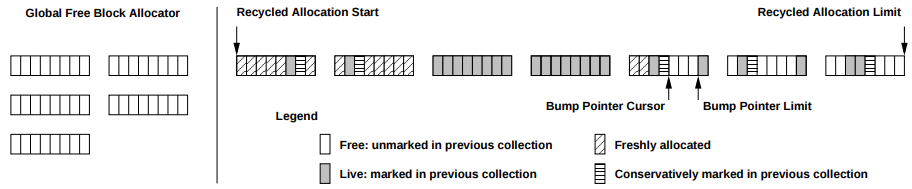
\includegraphics[width=1.0\linewidth]{images/immixHeap}
	\caption[Organizzazione dello heap]{Organizzazione dello heap in Immix}
	\label{fig:immixheap}
\end{figure}

\paragraph{Scelte implementative} 
\subparagraph{Politica di ''riciclaggio''.} Alla fine della pulizia ogni blocco è in uno e solo uno dei seguenti stati: libero, occupato o riciclabile. L'algoritmo marca come riciclabili quei blocchi con almeno \textbf{F} linee libere. Simulazioni hanno portato a scegliere F = 1.
\subparagraph{Politica di allocazione.} Immix alloca seguendo l'ordine degli indirizzi. Esistono altri ordinamenti per cercare di massimizzare la verosimiglianza di trovare blocchi liberi, ma i test hanno mostrato che quello scelto (che è molto semplice) è migliore. 
\subparagraph{Parallelismo.} L'implementazione è parallela e supporta più thread sia lato GC che lato applicazione. Tuttavia la pulizia non viene fatta concorrentemente all'esecuzione dell'applicazione. L'analisi dei blocchi è fatta in parallelo e permette race conditions nella marcatura degli oggetti (al più un oggetto verrà marcato più volte). Per evitare race conditions nell'aggiornamento di bit vicini vengono utilizzato interi byte per marcare le linee. Questo causa un overhead di 1/128, ma evita il bisogno di sincronizzazione. Questo approccio si comporta bene per thread veloci e non sincronizzati (sincronizzando solo i thread del GC) su sistemi monoprocessore o con due core. 
\subparagraph{Overflow Allocation on demand.} Allocare oggetti medi (più grandi di una linea) in blocchi frammentati può portare a sprecare grandi quantità di spazio. Per questo è utile utilizzare un \textit{overflow allocator}. Se Immix non riesce a soddisfare una richiesta rispetto allo spazio disponibile nel blocco corrente, ma ci sono blocchi totalmente liberi, l'oggetto viene allocato in uno di questi per evitare di sprecare spazio (e così l'oggetto è contiguo). Dato che spesso gli oggetti Java sono piccoli e che una linea può ospitare più oggetti, questa ottimizzazione permette di usare lo spazio in modo più efficiente.

\paragraph{Deframmentazione} \mbox{} \\
Un algoritmo mark-region non-moving è naturalmente soggetto a frammentazione. Sia l'evacuazione che il compattamento sono soluzioni ben conosciute, ma Immix utilizza un approccio più opportunistico. All'inizio di ogni pulizia determina se deframmentare o no a seconda del livello di frammentazione rilevato nelle precedenti analisi. 

Quando viene trovato un oggetto attivo in un blocco candidato, questo viene valutato. Viene evacuato solo se l'applicazione non l'ha bloccato e se lo spazio riservato per l'evacuazione non è terminato. Se un oggetto è inamovibile viene marcato come vivo e lasciato su quella locazione. Altrimenti, viene evacuato e sostituito con un puntatore alla nuova posizione. Se vengono trovati altri riferimenti dello stesso oggetto, questi vengono rimpiazzati con quel puntatore. Immix riserva un piccolo numero di blocchi completamente liberi come area per l'evacuazione: in generale lo spazio corrisponde al 2.5\%, ma può essere alzato a 3\% in condizioni di utilizzo intensivo.

\subparagraph{Selezione dei candidati.} Un sacco di euristiche possono essere utilizzate per selezionare i candidati alla deframmentazione. La strategia utilizzata è di tipo on demand. Se ci sono uno o più blocchi riciclabili non utilizzati dall'allocatore o se la precedente pulizia non ha liberato abbastanza spazio, Immix programma la deframmentazione per la prossima collezione. A questo punto vengono selezionati i blocchi con più buchi. Usa anche i dati raccolti nell'ultima analisi per selezionare quanti più blocchi possibili. Per calcolare queste stime velocemente vengono utilizzati due istogrammi basati sul conteggio dei buchi. Uno stima lo spazio richiesto (\textit{mark histogram}) e l'altro riflette lo spazio disponibile (\textit{available histogram}). Il primo è costruito in modo eager durante la pulizia alla fine di ciascuna collezione. Immix marca ogni blocco con il numero dei suoi buchi e aggiorna l'istogramma per indicare la distribuzione delle linee marcate nello heap in funzione del numero di buchi associati al blocco. Queste operazioni sono economiche e possono essere fatte alla fine di ogni collezione, anche se non sarà effettuata deframmentazione. Il secondo, invece, viene creato in modo lazy, solamente quando si decide di deframmentare. Ogni barra dell'istogramma riflette il numero di linee disponibili all'interno del blocco. Per identificare i candidati, Immix percorre l'istogramma, partendo dal punto di maggiore frammentazione. Incrementa lo spazio richiesto per il volume nella corrispondente barra del mark histogram e lo decrementa per il volume della barra dell'available histogram. Quando incontra un blocco per il quale la stima eccede il reale spazio disponibile, candida tutti i blocchi incontrati precedentemente per la deframmentazione. 

\subparagraph{Deframmentazione parallela.} Durante la deframmentazione è necessario sincronizzarsi per evitare che un oggetto venga evacuato in due posizioni per una race condition. 

\subparagraph{Pinning.} In alcune situazioni un'applicazione può chiedere che un oggetto non venga mosso. Sebbene questa funzionalità non sia direttamente supportata in Java, alcune implementazioni della VM possono richiederlo (ad esempio per migliorare la gestione del buffer per l'I/O da file). Di conseguenza Immix supporta direttamente questa possibilità, e non sposta gli oggetti per i quali l'applicazione fa pinning.

\paragraph{Valutazione} \mbox{} \\
Questa sezione analizza le prestazioni di Immix rispetto ad altri tre algoritmi di tre strategie diverse: \textbf{mark-sweep} (‘MS’, sweep-to-free-list), \textbf{semi-space} (‘SS’, evacuate),
e \textbf{mark-compact} (‘MC’, compact). 

Figura~\ref{fig:heapallocation} mostra l'efficienza in termini di spazio. Si nota che Immix si comporta generalmente meglio rispetto agli altri, tanto da essere sempre tra i migliori in termini di gestione delle allocazioni sullo heap. Come prevedibile SS, che occupa generalmente il doppio dello spazio a causa dell'evacuazione, è il peggiore. Immix si comporta generalmente meglio di MS, grazie alla gestione della memoria utilizzando due diverse granularità, ed ha un comportamento simile (e a volte addirittura migliore) di MC. Questo significa che la strategia di allocazione di Immix e tutte le ottimizzazioni inserite (gestione degli overflow e riciclaggio dei blocchi parzialmente occupati) consente di gestire lo spazio in modo migliore. Infatti, reclamare memoria a livello di linea consente di operare ad una granularità molto fine, sfruttando l'osservazione empirica che molto spesso gli oggetti Java sono di piccole dimensioni.
\begin{figure}[h]
	\centering
	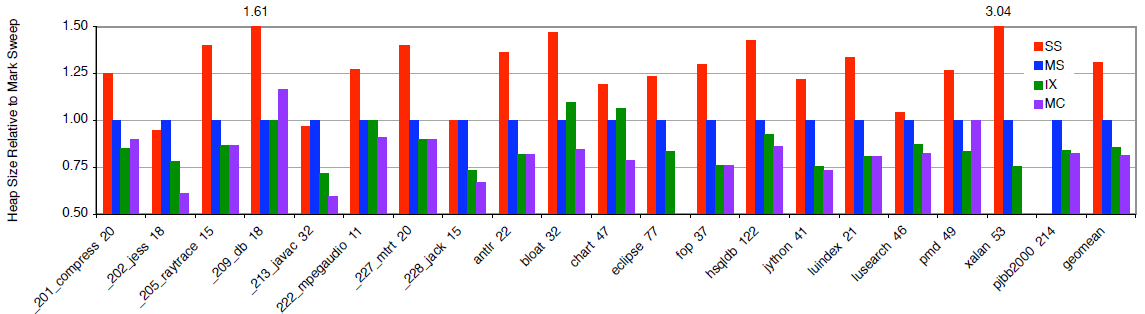
\includegraphics[width=0.7\linewidth]{heapAllocation}
	\caption[Efficienza di spazio]{Efficienza di spazio per vari algoritmi RTGC}
	\label{fig:heapallocation}
\end{figure}

Figura~\ref{fig:rtgc} mostra invece un confronto basato sulle performance dell'applicazione (Figura~\ref{fig:mutuatorPerformance}) e del processo di pulizia. (Figura~\ref{fig:fastCollection}). Come prevedibile la prima indica che le strategie SS e MC consentono all'applicazione prestazioni molto alte. Il motivo è, naturalmente, che queste due strategie allocano gli oggetti in maniera contigua, e di conseguenza l'applicazione ha tempi di esecuzione minori. Al contrario MS si comporta molto male, perché la sua politica causa molta frammentazione nella memoria. Immix si posiziona molto più in basso (e quindi ha un risultato molto migliore) di MS, arrivando quasi agli stessi livelli di SS e MC. Questo grazie alla deframmentazione opportunistica che viene eseguita on-demand solo quando è necessario. L'esecuzione on-demand consente ad Immix di non incorrere in un peggioramento di performance significativo durante la pulizia, come si può notare in Figura~\ref{fig:fastCollection}. Il tempo di collezione è praticamente uguale a quello di MS. Il risultato è coerente dato che il principio di base è lo stesso, l'unica variazione è la granularità a cui Immix opera. Al contrario MC e SS richiedono molto più tempo, come prevedibile dato che mantengono la memoria contigua ad ogni pulizia, e quindi incorrono in un overhead significativo.
\begin{figure}
	\centering
	\begin{subfigure}[b]{0.4\textwidth}
		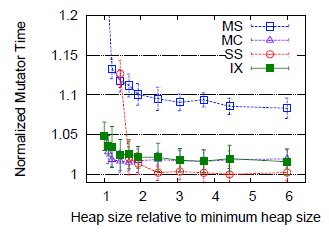
\includegraphics[width=\textwidth]{mutuatorPerformance}
		\caption{Performance dell'applicazione sotto GC}
		\label{fig:mutuatorPerformance}
	\end{subfigure}
	~
	\begin{subfigure}[b]{0.4\textwidth}
		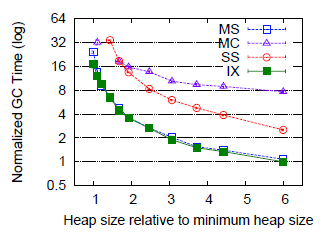
\includegraphics[width=\textwidth]{fastCollection}
		\caption{Tempo richiesto per la pulizia}
		\label{fig:fastCollection}
	\end{subfigure}
	\caption[Confronto di algoritmi RTCG]{Confronto di algoritmi RTCG basato sulle performance dell'applicazione e sul tempo di pulizia}\label{fig:rtgc}
\end{figure}

In definitiva, quindi, Immix raggiunge tutti e tre gli obiettivi necessari ad essere un buon algoritmo di RTGC: efficienza di allocazione (Figura~\ref{fig:heapallocation}), processo di collezione veloce (Figura~\ref{fig:fastCollection}) e non degrado delle performance dell'applicazione (Figura~\ref{fig:mutuatorPerformance}).

\subsection{Valutazione}
Figura~\ref{fig:fijicomp} mostra un confronto di varie VM progettate per sistemi real-time (fVM e WebSphere) e fortemente ottimizzate (Hotspot). 
\begin{figure}[h]
	\centering
	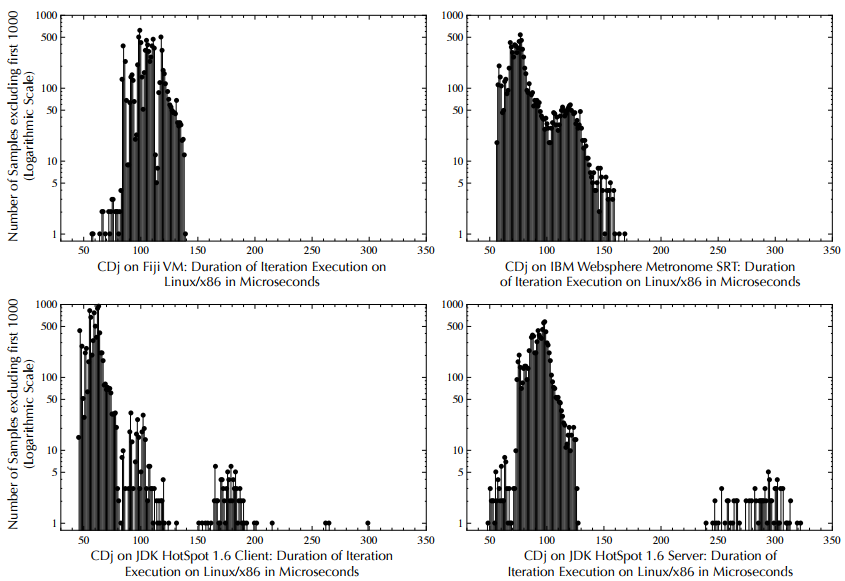
\includegraphics[width=0.8\linewidth]{images/fijicomp}
	\caption[Valutazione rispetto ad altre VM]{Valutazione di FijiVM rispetto ad altre VM}
	\label{fig:fijicomp}
\end{figure}

Si nota che Hotspot è decisamente più veloce rispetto a Fiji (37\% Server e 4.7\% Client), ma nel caso peggiore (quello realmente importante per sistemi real-time), Hotspot si comporta molto male (circa 185/200\% peggio di Fiji). Queste differenze sono causate dalle pause introdotte dalla GC, che non tiene conto della prevedibilità, ma cerca solo di ottimizzare il caso migliore. Rispetto a WebSphere, invece, Fiji si comporta meglio (nel caso peggiore) del 4\%, anche se in generale WebSphere è più veloce del 15\%. Tuttavia Fiji ha una distribuzione più stretta (calcolata rispetto alla differenza picchi/valli). Questo è un grande pregio, perché significa che la differenza tra il caso migliore e quello peggiore è più bassa.

Figura~\ref{fig:fijistartup} mostra l'evoluzione del caso peggiore per diverse VM. Il grafico è in qualche modo simile a quello mostrato in Figura~\ref{fig:performanceaotvsjit}. Hotspot e WebSphere utilizzano un compilatore JIT. Di conseguenza i tempo necessario al raggiungimento delle migliori prestazioni è variabile e più alto di quello di Fiji, che usa un compilatore AOT. Come detto precedentemente, le performance in generale saranno migliori per le altre VM (confermato da Figura~\ref{fig:fijicomp}), ma il tempo necessario per raggiungere quei livelli è alto e riduce il determinismo.
\begin{figure}[h]
	\centering
	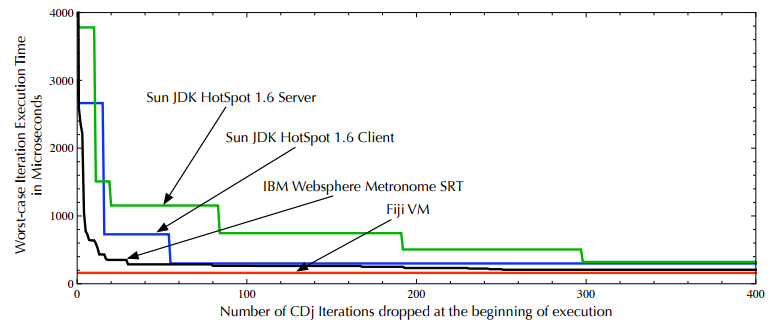
\includegraphics[width=0.8\linewidth]{images/fijistartup}
	\caption[Evoluzione del caso peggiore]{Evoluzione del caso peggiore per diverse VM}
	\label{fig:fijistartup}
\end{figure}
